\section*{Dudas de logística}
\begin{itemize}
    \item Llegar temprano.
\end{itemize}
% %%%%%%%%%%%%%%%%%%%%%%%%%%%%%%%%%%%%%%%%%%%%%%%%%%%%%%%%%%%%%%%%%%%%%%%%%%%%%%%%%%%%%%%%%%%%%%%%
\section{Análisis de aspectos empresariales}
\subsection{Tendencias}
\begin{itemize}
    \item Son predicciones del escenario futuro construías a partir del análisis de los hechos actuales y de acontecimientos históricos. 
    \item Las tendencias permiten predecir y especular por ende permiten mejorar las decisiones empresariales.
    \item Microprocesos: cuatro resultados organizados grandiosos.
        \begin{itemize}[label=$\downarrow$]
            \item Análisis de la situación actual:
                \begin{enumerate}
                    \item FE 
                    \item Industria
                    \item La empresa 
                \end{enumerate}
            
            \item Hechos históricos relevantes de la industria:
            
            \item Tendencias:
                \begin{itemize}
                    \item Ejecución Innovación 
                    \item Emprendimiento: Hay dos tipos de emprendimiento
                        \begin{enumerate}
                            \item Intraemprendimento: emprender desde adentro de las compañías (interno). 
                            \item Emprendimiento: emprender desde afuera independiente (Independiente externo).
                        \end{enumerate}
                \end{itemize}

            \item Oportunidades de negocios
        \end{itemize}
\end{itemize}
\begin{figure}[htbp]
    \centering
    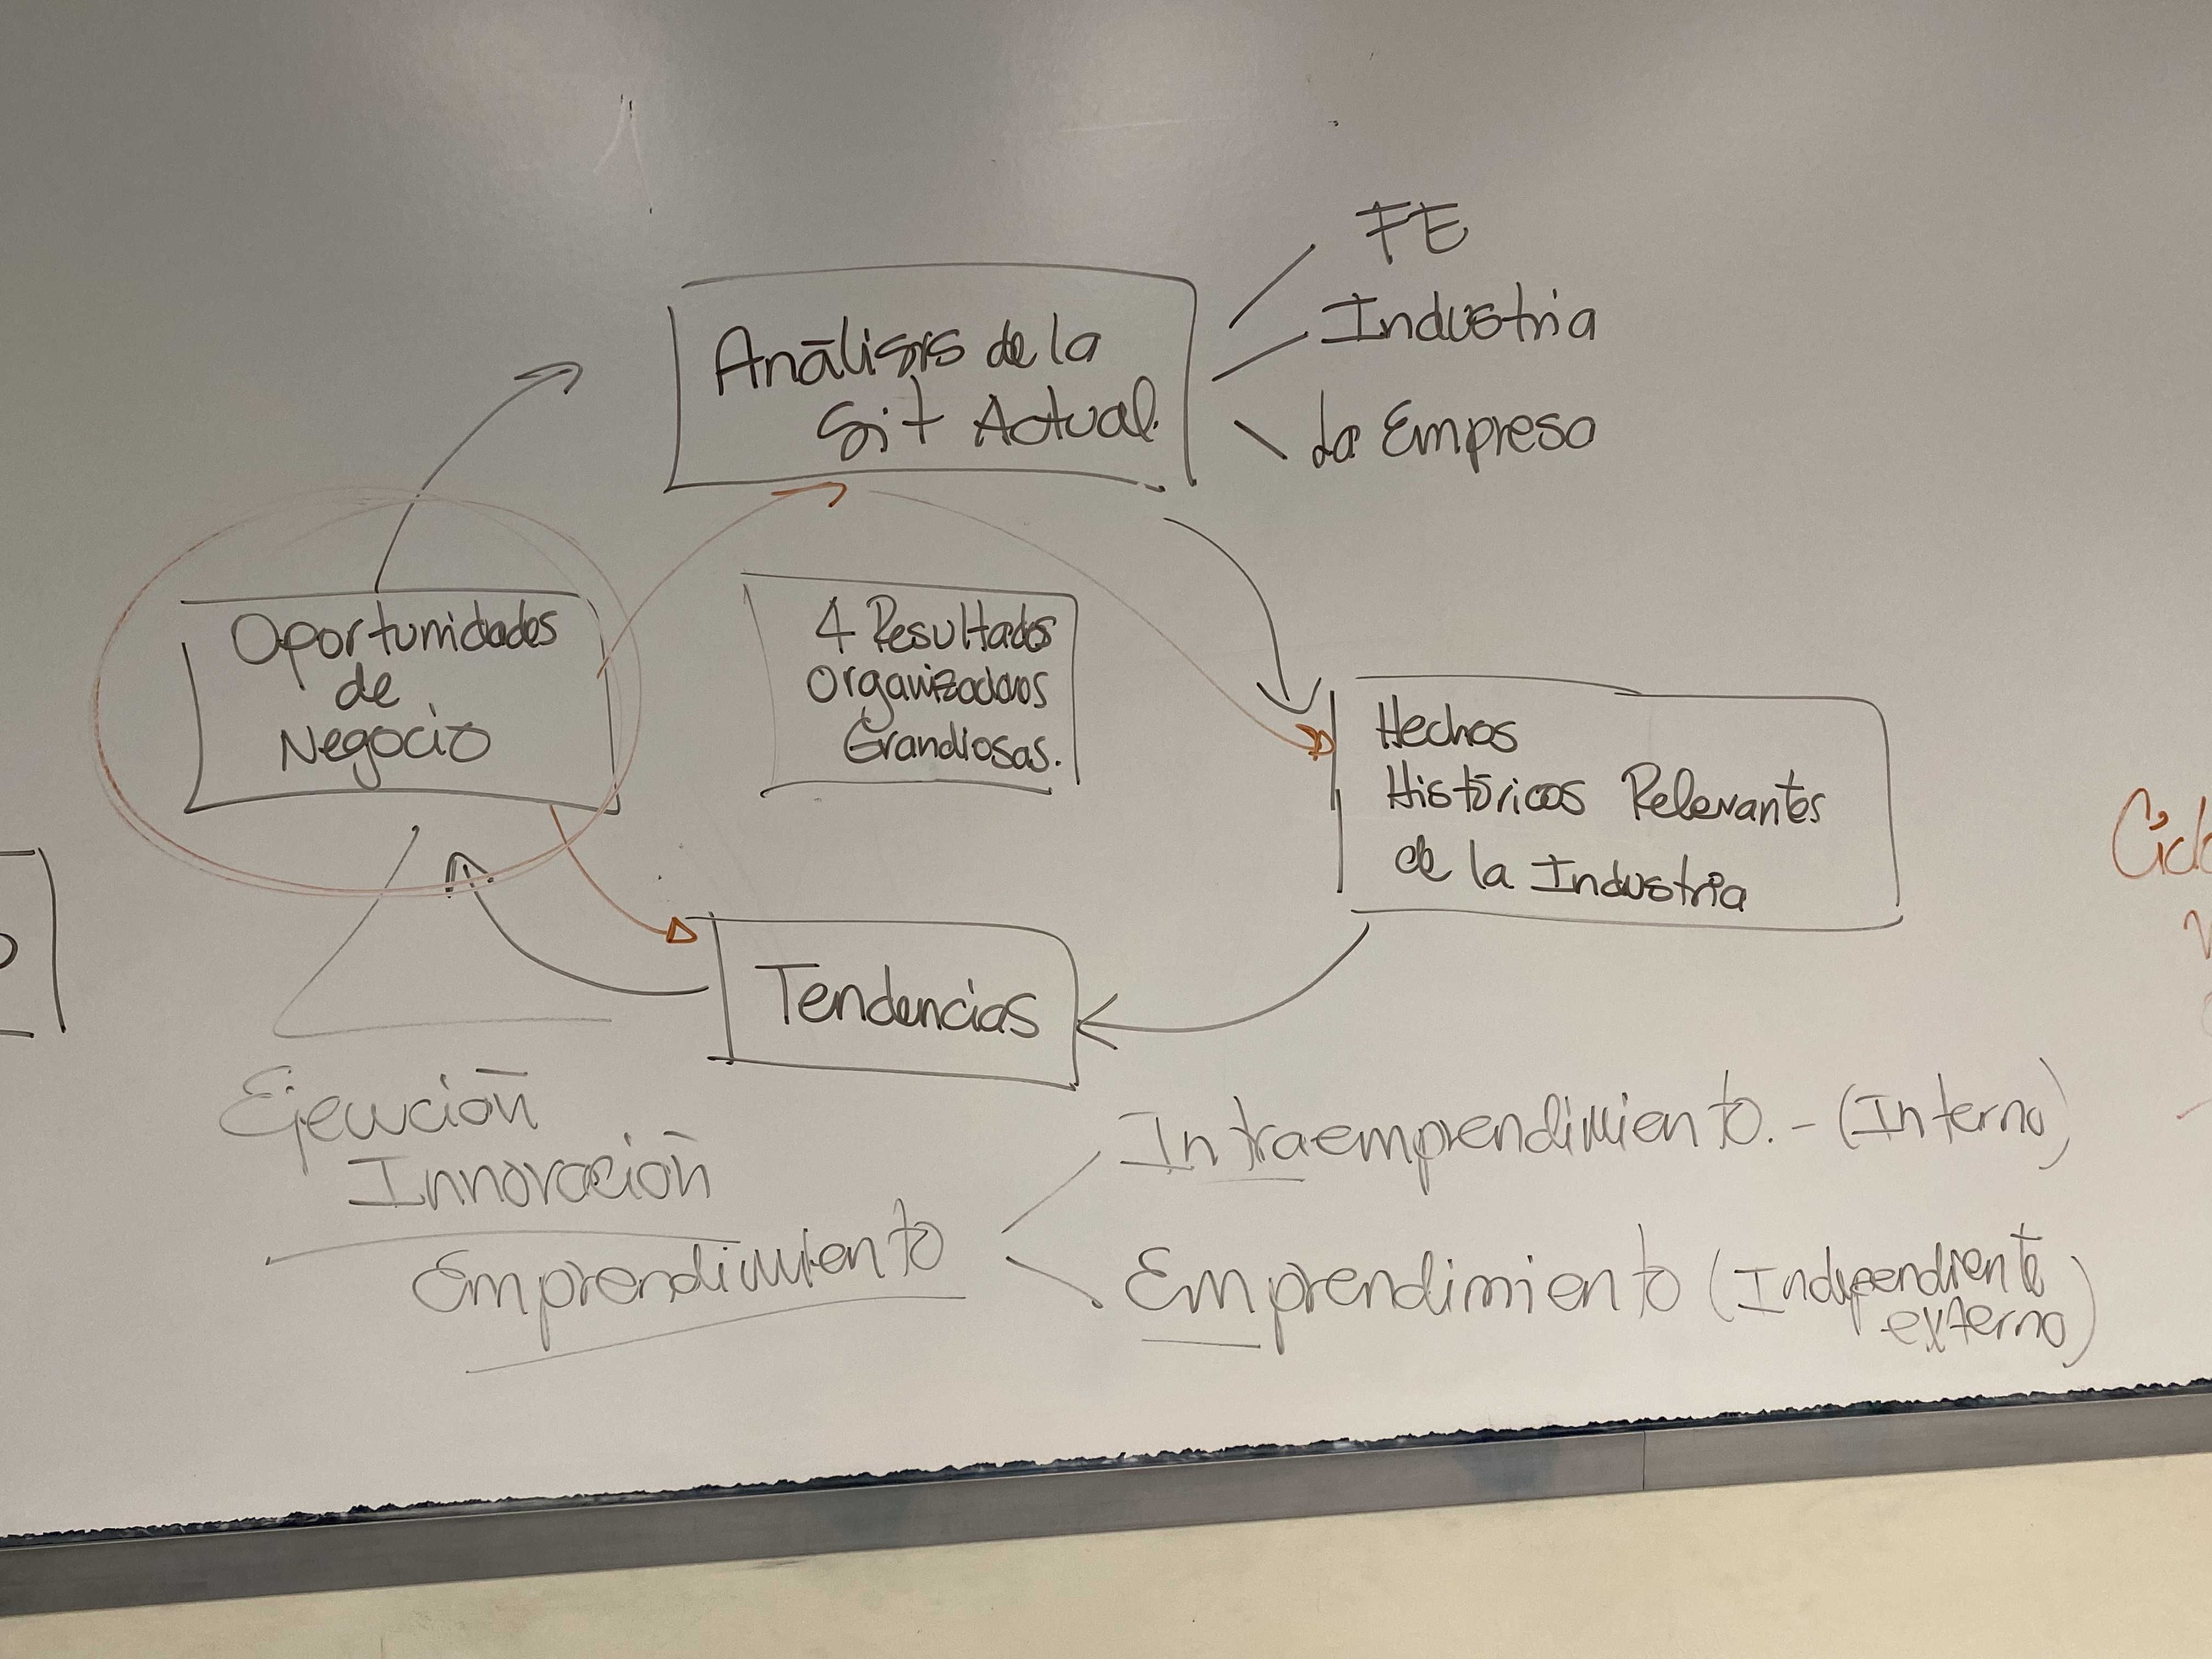
\includegraphics[width=6cm]{Clases/Images/2020-01-15-Empresarialidad.jpeg}
    \caption{Aspectos empresariales}
    \label{}
\end{figure} 
%%%%%%%%%%%%%%%%%%%%%%%%%%%%%%%%%%%%%%%%%%%%%%%%%%%%%%%%%%%%%%%%%%%%%%%%%%%%%%%%%%%%%%%%%%%%%%%%
\subsection{\emph{\textbf{Recordar lo siguiente: }El único constante es el cambio.}}
\begin{itemize}
    \item El gobierno no es de confianza, según las cifras se ha disminuido el nivel de confianza al gobierno.
    \item Hay un cambio a partir de 1950 por los avances tecnológicos, conforme sale esta nueva tecnología lo que dieron a la sociedad un boost que cambiaron las reglas, se dieron fenómenos de destrucción creativa y de innovación.
\end{itemize}
%%%%%%%%%%%%%%%%%%%%%%%%%%%%%%%%%%%%%%%%%%%%%%%%%%%%%%%%%%%%%%%%%%%%%%%%%%%%%%%%%%%%%%%%%%%%%%%%
\subsection{ Globalización: La aldea global.}
\begin{itemize}
    \item Fue este boost que se dio a partir de 1950.
    \item En 1989 cae el muro de Berlin, est hecho da a inicio a el fenómeno de la globalización.
    \item Factor externo $\rightarrow$ Tecnología.
    \item Cuando cae el muro de Berlin se derriba el muro de separación entre los socialistas y los capitalistas. Se eliminan todas las barreras económicas y políticas con esta información se puede comercializar a nivel global.
    \item \emph{\textbf{Definición de ``globalización":} Es el resultado de una seria de cambios irreversibles y constantes generados por el desarrollo tecnológico.}
    \item Línea de tiempo: 
        \begin{center}
            \begin{tabular}{ | p{15cm} | }
                \hline
                    1989 - Cae el muro de Berlín \\ 
                    \hline
                    1992 - Clinton da acceso a email solo a gobierno  \\ 
                    \hline
                    1995 - Netscape crea un browser \\ 
                    \hline
                    1998 - PayPal surge e introduce un sistema de cobro y pago virtual \\ 
                    \hline
                    2000 - Boom outsorcing, India se vuelve era el principal proveedor de fibra óptica de EEUU \\ 
                    \hline
                    2001 - Offshoring la mano de obra se va a China por ser más barato, China entra con la OMC(Organización Mundial del Comercio) \\ 
                    \hline
                    2004 - Open Source code, Software con Open Source Code Available  \\ 
                    \hline
                    2005 - Todo el mundo tenía conectividad por medio del WWW \\ 
                \hline
            \end{tabular}
        \end{center}
    
    \item Geoeconomía: \emph{\textbf{Definición de ``geoeconomía":} es el nuevo concepto económico que surge a partir de la globalización.}
    \item \emph{\textbf{Recordar lo siguiente: }Las personas tardaron en agarrar confianza en el internet. La gente no tenía nada de confianza. PayPal crea alianzas con India por medio de CallCenter esto lo introducen las aerolíneas.}
    \item \emph{\textbf{Definición de ``OutSorcing":} Contratar a servicios especializados, tercerizar. \emph{\textbf{Ejemplo: }Los CallCenters en India es una forma de tercerizar o offshoring.}}
    \item \emph{\textbf{Definición de ``Offshoring":} Montar procesos de producción o fabricación fuera del territorio de orígen.}
    \item \textbf{Importante:} Analizar un hecho histórico (globalización) y un factor externo (tecnología).
\end{itemize}
%%%%%%%%%%%%%%%%%%%%%%%%%%%%%%%%%%%%%%%%%%%%%%%%%%%%%%%%%%%%%%%%%%%%%%%%%%%%%%%%%%%%%%%%%%%%%%%%

\section{Ciclo de vida}
\subsection{Punto inicial - StartUps}
\begin{itemize}
    \item Empieza despacio, los ingresos son bajos y luego empiezan a crecer.
    \item Invierto en mercadeo.
    \item Competitividad, precio, calidad, proveedor. 
    \item Tener bastantes puntos de venta.
\end{itemize}

\subsection{Crecimiento - Expansión}
\begin{itemize}
    \item Ya tiene clientes profundamente leales
\end{itemize}

\subsection{Madurez}
\begin{itemize}
    \item Se mantiene bien por un tiempo y se prepara para estallar.
\end{itemize}

\subsection{Tiempo}
\begin{itemize}
    \item Se da un punto de innovación o de decline.
    \item Aquí se puede inicializar de nuevo la etapa de inicial.
\end{itemize}



% \begin{figure}[htbp]
%     \centering
%     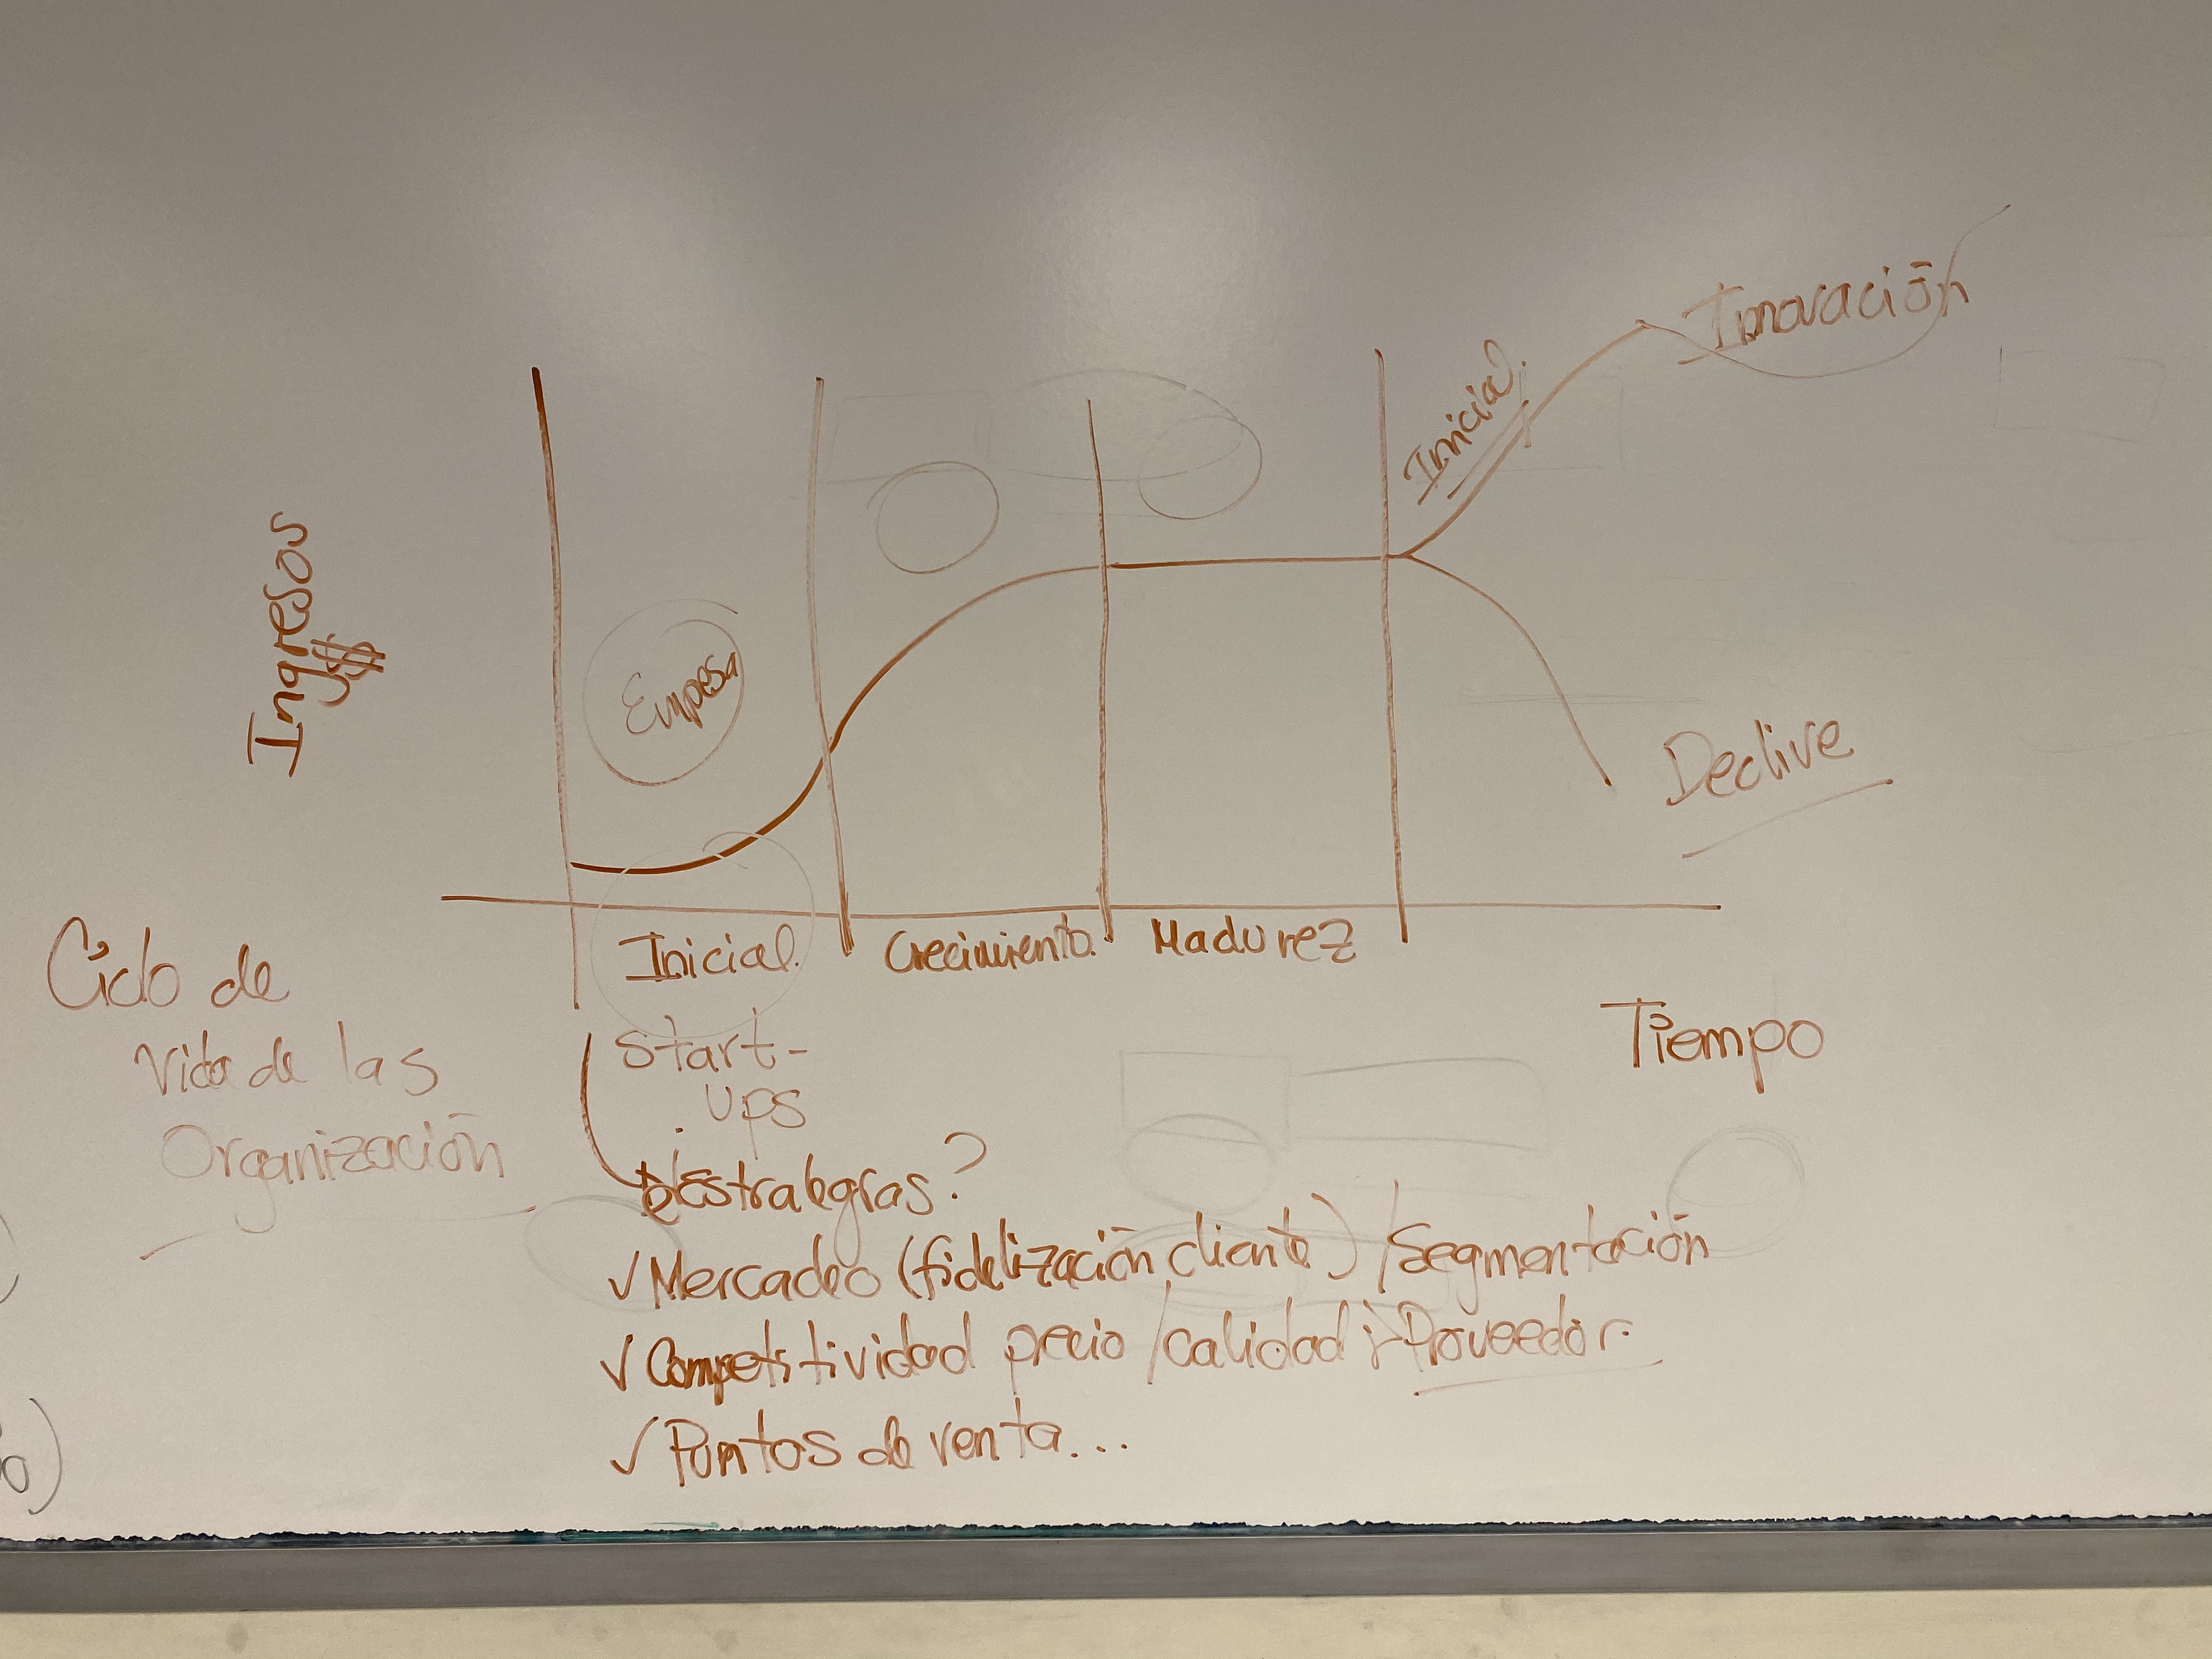
\includegraphics[width=6cm]{Clases/Images/2020-01-15-CicloDeVidaOrganizacion.jpeg}
%     \caption{Ciclo de vida de las organizaciones}
%     \label{}
% \end{figure} 


\section*{Tarea}
\begin{itemize}
    \item Investigar las etapas e identificar una empresa que está en una de estas etapas.
\end{itemize}   
